\documentclass{article}
\usepackage{graphicx}
\usepackage{float}
\usepackage[acronym]{glossaries}
\usepackage{fullpage}

\loadglsentries{acronyms}
\makeglossaries

\begin{document}

\begin{tabular}{rl}
  \textbf{Lab 8:} & DC Generators \\
  \textbf{Performed:} & March 26, 2013 \\
  \textbf{Partners:} & Rawley Dent \\ & Charles Pittman \\
  \textbf{Instructor:} & Dr. Weatherford
\end{tabular}

%\setlength\parindent{0pt}

\section*{Abstract}

In this experiment, the basic principles of operation of DC generators were studied. The output voltage (terminal
voltage $V_T$) and output current (line current $I_L$) relationship for a separately excited generator, shunt 
connected generator, and cumulatively compounded connected generator were studied with various loads, from no-load 
down to 57 \Omega. 

\section*{Results}

\begin{figure}[H]
  \centering
    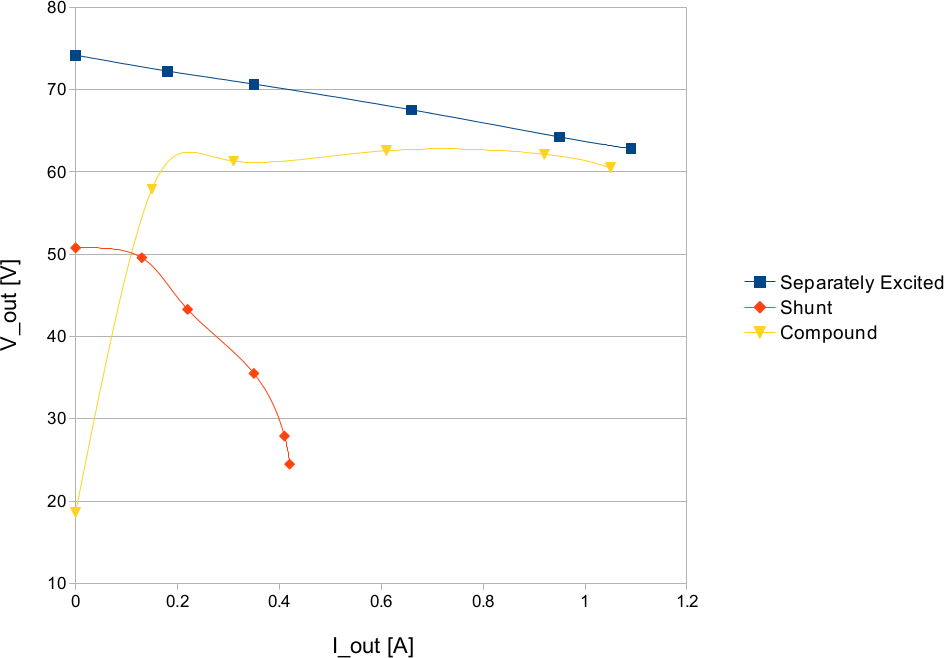
\includegraphics[width=0.8\textwidth]{img/graph}
    \caption{\textbf{Comparison}}
    \label{fig:graph}
\end{figure}

\section*{Conclusions}

For DC motors, the teminal characteristics are induced torque and motor speed. However, for DC generators the 
terminal characteristics are terminal voltage and line current, that is the output voltage and output current. 
In the figure above the terminal characteristics of a separately excited, shunt connected, and compound connected
DC generator are compared. The terminal characteristics of a separately excited generator can be seen to be a straight 
line. As the load was increased in the experiment, the line current and thus the armature current increased. From 
Kirchoff's voltage law $V_T = E_A - I_AR_A$ the terminal voltage will thus decrease as line current increases, and 
in a linearly fashion since the internal generated voltage $E_A$ is independent of the armature current $I_A$. The 
terminal characteristics of a shunt connected generator are similar to that of a separately excited generator. However,
in a shunt generator the amount of field current depends of the terminal voltage. As the terminal voltage decreases then 
so does the field current. This causes the flux to decrease which then causes the internal genearated voltage $E_A$ to 
decrease and thus the terminal voltage decreases even more as the output current increases. The terminal characteristics 
of a cumulatively compounded generator consist of two terminal voltage effects which oppose each other. As the load 
increased, the output current and thus the armature current increased. From Kirchoff's voltage law 
$V_T = E_A - I_A(R_A + R_S)$ as the armature current increases, the terminal voltage decreases. However, since the 
armature current increases then the total magnetomotive force increases which increases the flux in the 
generator, which in turn increases the internal generated voltage $E_A$ and thus increases the terminal voltage. Thus,
the two terminal voltage effects oppose each other with one or the other predominating.
\end{document}
